\documentclass[a4paper]{article}
%\usepackage[singlespacing]{setspace}
\usepackage[onehalfspacing]{setspace}
%\usepackage[doublespacing]{setspace}
\usepackage{geometry} % Required for adjusting page dimensions and margins
\usepackage{amsmath,amsfonts,stmaryrd,amssymb,mathtools,dsfont} % Math packages
\usepackage{tabularx}
\usepackage{colortbl}
\usepackage{listings}
\usepackage{amsmath}
\usepackage{amssymb}
\usepackage{enumerate}
\usepackage{enumitem}
\usepackage{amsthm}
\usepackage{subcaption}
\usepackage{float}
\usepackage[table,xcdraw]{xcolor}
\usepackage{tikz-qtree}
\usepackage{forest}
\usepackage{changepage,titlesec,fancyhdr} % For styling Header and Titles
\pagestyle{fancy}
\renewcommand{\headrulewidth}{0.5pt} % Linienbreite anpassen, falls gewünscht
\renewcommand{\headrule}{
    \makebox[\textwidth]{\rule{1.0\textwidth}{0.5pt}} 
}
\usepackage{amsmath}
\pagestyle{fancy}
\usepackage{diagbox}
\usepackage{xfrac}

\usepackage{pgfplots}
\usepackage{pgfplotstable}
\pgfplotsset{compat=1.18}

\usepackage{enumerate} % Custom item numbers for enumerations

\usepackage[ruled]{algorithm2e} % Algorithms

\usepackage[framemethod=tikz]{mdframed} % Allows defining custom boxed/framed environments

\usepackage{listings} % File listings, with syntax highlighting
\lstset{
	basicstyle=\ttfamily, % Typeset listings in monospace font
}

\usepackage[ddmmyyyy]{datetime}


\geometry{
	paper=a4paper, % Paper size, change to letterpaper for US letter size
	top=3cm, % Top margin
	bottom=3cm, % Bottom margin
	left=2.5cm, % Left margin
	right=2.5cm, % Right margin
	headheight=25pt, % Header height
	footskip=1.5cm, % Space from the bottom margin to the baseline of the footer
	headsep=1cm, % Space from the top margin to the baseline of the header
	%showframe, % Uncomment to show how the type block is set on the page
}
\lhead{\vspace{0.5\baselineskip}Übungsblatt 3}
\chead{\bfseries{Einführung in Verteilte Systeme\\Sommersemester 2025}}
\rhead{\vspace{0.5\baselineskip}Werner, 7987847}
\fancyheadoffset[R]{0cm}

\begin{document}
\setcounter{section}{3}
\subsection{}
Was sind die Vorteile von Glasfaser gegenüber Kupfer als Übertragungsmedium? Gibt es auch Nachteile?\\\\
\underline{Vorteile:}
\begin{itemize}
    \item \textbf{Geschwindigkeit}: Kommunikation über Glasfaser läuft mit Lichtgeschwindigkeit im jeweiligen Medium (wenn Verzögerungen von Verstärkern, dem Medium selbst usw. vernachlässligt werden)
    \item \textbf{Signalparalelität}: Glasfaser kann mehrere Verschiedene Signale mit verschiedenen Lichtfrequenzen auf der gleichen Leitung transportieren. Das ermöglicht eine imens größere Bandbreite
    \item \textbf{Unempfindlichkeit}: Glasfaser wird nicht durch elektromagnetische Felder oder ähnliches gestört
    \item \textbf{geringer Signalverlust}: Auf langen Strecken hält sich das Signal deutlich länger
\end{itemize}
\underline{Nachteile:}
\begin{itemize}
    \item \textbf{Empfindlichkeit}: Glasfaser ist filigran und Knicke führen zum direkten Signalbruch. Dadurch ist der Einbau und die Nachrüstung teurer und aufwenidger
\end{itemize}

\subsection{}
Ein Koaxialkabel vom Typ $RG-58\,(50 \Omega)$ sei mit verschiedenen weiteren Koaxialkabeln unbekannten Typs verlängert worden. Bekannt ist dabei die Ausbreitungsgeschwindigkeit des Signals im Kabel von $c = 200 000 km/s$. Die Kabelstrecke sei auf beiden Seiten reflexionsfrei terminiert. Da Probleme bei der Datenübertragung auftreten, wird vermutet, dass eine der Verlängerungen einen falschen Impedanzwert hat. Um das zu untersuchen, wird am Anfang der Kabelstrecke ein periodischer Rechteckpuls angelegt.\\
An der gleichen Stelle wird das Signal auf der Leitung mit folgendem Ergebnis gemessen (idealisierte Darstellung):
\begin{center}
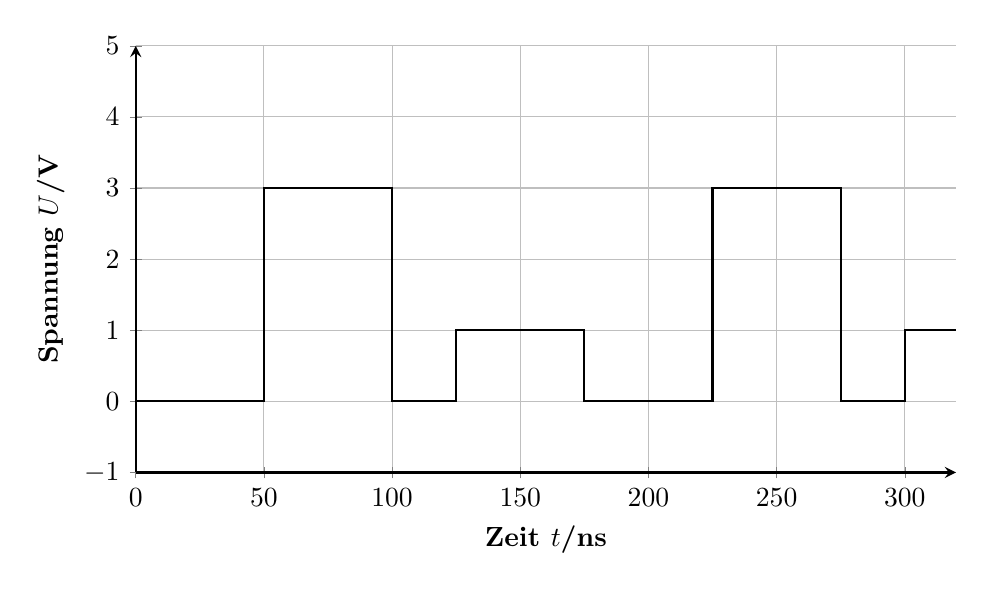
\begin{tikzpicture}
  \begin{axis}[
    width=12cm,
    height=7cm,
    grid=both,
    xlabel={\textbf{Zeit $t$/ns}},
    ylabel={\textbf{Spannung $U$/V}},
    xmin=0, xmax=320,
    ymin=-1, ymax=5,
    xtick={0,50,...,300},
    ytick={-1,0,...,5},
    thick,
    domain=0:320,
    samples=100,
    enlargelimits=false,
    axis lines=left
  ]

  \addplot[
    black,
    thick
  ] coordinates {
    (0,0)
    (50,0)
    (50,3)
    (100,3)
    (100,0)
    (125,0)
    (125,1)
    (175,1)
    (175,0)
    (225,0)
    (225,3)
    (275,3)
    (275,0)
    (300,0)
    (300,1)
    (320,1)
  };
  \end{axis}
\end{tikzpicture}
\end{center}
\begin{enumerate}[label=\alph*)]
    \item Welche Frequenz hat das angelegte Rechtecksignal?\\
    Wir erkennen, dass der Spike auf 3V zwischen \texttt{50-100ms} und \texttt{225-275ms} und das darauffolgende Signal gleich sind, dadurch können wir die Periodenlänge $T$ bestimmen: $T = 225ns - 50ns = 175ns = 175 \cdot 10^{-9}s$\\
    Damit können wir die Frequenz berechnen: $f = \frac{1}{T} = \frac{1}{175 \cdot 10^{-9}s} \approx 5714285,714Hz \approx 5.71GHz$
    \item Nach welcher Kabellänge vermuten Sie das falsche Anschlusskabel?
    \begin{itemize}
        \item Ausbreitungsgeschwindigkeit: $c = 200000km/s = 2 \cdot 10^{8}m/s$
        \item Spannungsdelta I : $3V \Rightarrow 0V$ bei $100ms$
        \item Spannungsdelta II: $0V \Rightarrow 1V$ bei $125ms$
    \end{itemize}
    $\Rightarrow$ Verzögerung $t_{dif} = 125ms - 100ms = 25ms$\\
    Das Signal verläuft hin und zurück, daher ist $t_{single\_dif} = 25ms \div 2 = 12.5ms$\\
    Somit erwarten wir das falsche Anschlusskabel bei $d = c \cdot t_{single\_dif} = 2 \cdot 10^{8}m/s \cdot 12.5 \cdot 10^{-9}s = 2.5m$
    \item Berechnen Sie den Impedanzwert des falschen Kabels (unter Annahme verlustfreier Kabel).\\
    \begin{itemize}
        \item reflektierte Spannung: $U_r = 1V$
        \item eingehende Spannung: $U_{in} = 3V$
        \item Kabelwiederstand: $R_k = 50\Omega$ für beide Kabel
    \end{itemize}
    Der Reflexionskoeffizient lautet dann \[\gamma = \frac{z - R_k}{z - R_k} \overset{!}{=} \frac{U_r}{U_{in}} \Rightarrow \frac{1}{3} = \frac{z - 50\Omega}{z - 50\Omega} \Leftrightarrow z = 100\Omega\]
\end{enumerate}
\clearpage
\subsection{}
Ein differentielles Signal werde zunächst über ein UTP-Kabel (Unshielded Twisted Pair) übertragen und gehe an einem Steckverbinder auf ein Leiterbahnpaar über. Beim Übergang sollen
möglichst keine Reflexionen entstehen. Dazu soll auf beiden Teilen der Übertragungsstrecke eine differentielle Impedanz von $Z = 100 \Omega$ erreicht werden.
\begin{enumerate}[label=\alph*)]
    \item Das UTP-Kabel bestehe aus einem Paar direkt aneinander angrenzender isolierter Kupferleiter. Jeder der Kupferleiter habe einen Durchmesser von $d = 0,5 mm$. Der Abstand $a$ des Leiterpaares (vgl. Vorlesung) ergibt sich dann aus der Dicke $d_i$ der Isolation: $a = d+2\cdot d_i$.\\\\
    Für die Permeabilitätszahl in den beteiligten Materialen gelte $\mu_r \approx 1,0$. Für die Permittivitätszahl gelte in der Materialanordnung ein effektiver Wert von $\epsilon_r \approx 2,6$.\\\\
    Wie dick muss der Isolationsmantel der Adern gewählt werden, damit das Kabel die gewünschte differentielle Impedanz von $Z = 100 \Omega$ aufweist?

    Ein UTP-Kabel mit Kupferleitern hat den Durchmesser \( d = 0.5mm \). Der Abstand der Leiter beträgt:
    \[
    a = d + 2d_i
    \]
    
    Für ein ungeschirmtes verdrilltes Paar ergibt sich die differentielle Impedanz näherungsweise zu:
    \[
    Z \approx \frac{120\,\Omega}{\sqrt{\varepsilon_r}} \cdot \ln\left( \frac{a}{d} \right)
    \]
    
    Einsetzen von \( a = d + 2d_i \) ergibt:
    \[
    Z = \frac{120}{\sqrt{2{,}6}} \cdot \ln\left(1 + \frac{2d_i}{d} \right)
    \]
    
    \textbf{Ziel:} \( Z = 100\mu m \)
    
    \vspace{1em}
    
    \textbf{Berechnung:}\\
    $
    \frac{120}{\sqrt{2{,}6}} \approx 74{,}42 \\
    \Rightarrow \quad \ln\left(1 + \frac{2d_i}{d} \right) = \frac{100}{74{,}42} \approx 1{,}344 \\
    \Rightarrow \quad 1 + \frac{2d_i}{d} = e^{1{,}344} \approx 3{,}833 \\
    \Rightarrow \quad \frac{2d_i}{d} = 2{,}833 \\
    \Rightarrow \quad d_i = \frac{2{,}833 \cdot d}{2} = \frac{2{,}833 \cdot 0.5mm}{2} \approx 0.708mm
    $\\
    \clearpage
    \item Für die Single-Ended-Impedanz $Z_N$ einer Leiterbahn auf der Oberfläche einer Leiterplatte (surface microstrip, siehe Vorlesung) gilt die Näherungsformel
    \[Z_N=\frac{87 \Omega}{\sqrt{\epsilon_r + 1,41}}ln\frac{5.98D}{0,8b+d}\]
    für $0,5 < D/b < 3$ mit der Dicke $d$ und Breite $b$ der Leiterbahn und dem Abstand $D$ zur nächsten Massefläche.\\\\
    Die differentielle Impedanz zweier auf der Oberfläche mit dem Abstand $s$ parallel laufender Leiterbahnen lässt sich näherungsweise aus der Single-Ended-Impedanz $Z_N$ bestimmen als
    \[Z_{diff}=2\cdot Z_N\left(1-0.48 exp\left(-0.96\frac{s}{D}\right)\right)\]
    Beim vorliegenden Leiterplattenprozess gelte: $D = 150 \mu m, d = 35 \mu m, \epsilon_r = 4,3$.\\\\
    Wie groß muss der Abstand $s$ zwischen zwei Leiterbahnen der Breite $b = 150 \mu m$ sein, damit das Signal reflexionsfrei vom Kabel übergehen kann?\\\\
    \textbf{Gegeben:}

    Die Single-Ended-Impedanz einer Leiterbahn auf einer Leiterplatte ist näherungsweise gegeben durch:
    \[
    Z_N = \frac{87\,\Omega}{\sqrt{\varepsilon_r + 1{,}41}} \cdot \ln\left( \frac{5{,}98D}{0{,}8b + d} \right)
    \]
    
    Für den vorliegenden Fall gelten:
    \[
    \varepsilon_r = 4{,}3, \quad D = 150\mu m, \quad d = 35\mu m, \quad b = 150\mu m
    \]
    
    \textbf{Einsetzen:}
    \[
    Z_N = \frac{87}{\sqrt{4{,}3 + 1{,}41}} \cdot \ln\left( \frac{5{,}98 \cdot 150}{0{,}8 \cdot 150 + 35} \right)
    = \frac{87}{\sqrt{5{,}71}} \cdot \ln\left( \frac{897}{155} \right)
    \]
    
    \[
    \Rightarrow Z_N \approx \frac{87}{2{,}39} \cdot \ln(5{,}79) \approx 36{,}4 \cdot 1{,}756 \approx 63,9\Omega
    \]
    
    \vspace{1em}
    
    Die differentielle Impedanz ergibt sich zu:
    \[
    Z_{\text{diff}} = 2 \cdot Z_N \cdot \left(1 - 0{,}48 \cdot e^{-0{,}96 \cdot \frac{s}{D}} \right)
    \]
    
    \textbf{Gesucht:} Abstand \(s\), sodass \(Z_{\text{diff}} = 100\Omega\)
    
    \vspace{1em}
    
    \textbf{Berechnung:}\\
    $
    100 = 2 \cdot 63{,}9 \cdot \left(1 - 0{,}48 \cdot e^{-0{,}96 \cdot \frac{s}{150}} \right) \\
    \Rightarrow \quad \frac{100}{127{,}8} = 1 - 0{,}48 \cdot e^{-0{,}96 \cdot \frac{s}{150}} \\
    \Rightarrow \quad 0{,}782 = 1 - 0{,}48 \cdot e^{-0{,}96 \cdot \frac{s}{150}} \\
    \Rightarrow \quad 0{,}218 = 0{,}48 \cdot e^{-0{,}96 \cdot \frac{s}{150}} \\
    \Rightarrow \quad e^{-0{,}96 \cdot \frac{s}{150}} = \frac{0{,}218}{0{,}48} \approx 0{,}454 \\
    \Rightarrow \quad -0{,}96 \cdot \frac{s}{150} = \ln(0{,}454) \approx -0{,}789 \\
    \Rightarrow \quad s = \frac{150 \cdot 0{,}789}{0{,}96} \approx 123,3\mu m
    $
\end{enumerate}
\textbf{Hinweis:} Die Permittivität $\epsilon$ eines Materials kann als Produkt einer Permittivitätszahl $\epsilon_r$ und der elektrischen Feldkonstante $\epsilon_0$ geschrieben werden: $\epsilon = \epsilon_r \cdot \epsilon_0$. Analog gilt für die magnetische Permeabilität $\mu$ mit der Permeabilitätszahl des Materials $\mu_r$ und der magnetischen Feldkonstante $\mu_0: \mu = \mu_r \cdot \mu_0$.
\end{document}
